% You should title the file with a .tex extension (hw1.tex, for example)
\documentclass[a4paper, 12pt]{report}

\usepackage{amsmath}
\usepackage{amssymb}
\usepackage{tabularx}
\usepackage{fancyhdr}
\usepackage{minted}
\usepackage{amsthm}        
\usepackage{graphicx}
\usepackage{hyperref}
\hypersetup{
    colorlinks=true,
    linkcolor=black,
    filecolor=magenta,      
    urlcolor=cyan,
    pdfpagemode=FullScreen,
}

\renewcommand\qedsymbol{$\blacksquare$}


\graphicspath{ {./pictures} }

\usepackage[margin=1in]{geometry}

\newcommand{\question}[2] {\vspace{.25in} \hrule\vspace{0.5em}
\noindent{\bf #1: #2} \vspace{0.5em}
\hrule \vspace{.10in}}
\renewcommand{\part}[1] {\vspace{.10in} {\bf (#1)}}

\newcommand{\myname}{Krittin Nisunarat}
\newcommand{\myhwnum}{1}
\newcommand{\mySubject}{ICCS315 Applied Algorithms}

\setlength{\parindent}{20pt}
\setlength{\parskip}{5pt plus 1pt}
 
\pagestyle{fancyplain}
\lhead{\fancyplain{}{\textbf{Project}}}      % Note the different brackets!
\rhead{\fancyplain{}{\myname}}
\chead{\fancyplain{}{\mySubject}}

\title{
	{
\includegraphics[width=80mm,scale=0.5]{MUIC_Logo_Eng_Center.png}} \\
	{\textbf{\mySubject}}\\
	{\large Assignment \myhwnum \ Report}\\
}
\author{
	{\textbf{Written by}} \\ 
	{Krittin Nisunarat 6280782}
}
\date{30 Jan 2022}
\thispagestyle{plain}


\begin{document}
\maketitle
\tableofcontents

\chapter{Resizeable Arrays}

Traditionally, resizable array has a high amortized cost depending on $\alpha$ for expansion and shrinking. HAT array theoretically fares
with a constant amortized cost on expansion and shrinking. Our goal is to perform teh benchmarking of the actual implementation of 
traditionaly resizable array and Sitarski's HAT array.

\section{Set up}

Both of data structure implementations are written in C++ which runs on ubuntu server. 
The actual implement is in \href{https://github.com/sudo-lucifer/applied-algo-hw1/tree/main/hat_array}{Github}.

\section{Append latency}

In this section, the cost of appending one key to the array mainly comes from reading memory. 
On tradditional resizable array, pushing new key to the back costs approximatetly 47 cycles
from reading memory pointer which needs to be conducted at most the entire array. On the other hand,
Sitarski's HAT array takes less cycle per apeend operation since the entire array is separated 
into $b$ size where $b$ where $b = 2^k$.

\begin{figure}[h]
        \centering
        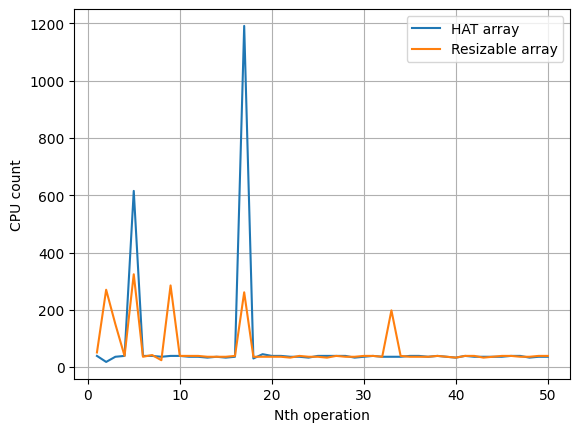
\includegraphics[width=0.5\textwidth,scale=0.2]{append_latency_output.png}
        \caption{\label{fig:append-latency} Benchmark of each append costs}
\end{figure}

Figure \ref{fig:append-latency} shows the cost of each append out of 50 append operations.
Tradditional resizable array shows up to stike CPU cycle more on each operation since the expansion
happens more often than HAT array. However, HAT array costs significantly higher cycle because the 
resizing needs to be done in both levels combine with copying data over.

In conclusion, traditional resizable array takes more cycle to access memory and append new day than
HAT array. On the expansion, tradditional resizable array is better than HAT array.

\section{Overall throughput}

In section 1.1, I have shown append latency which conclude to have different benefits.
For this benchmark, I will test inserting 50 elements to both tradditional resizable array and
HAT array. As a consequence, resizable array takes 1153 cycles on average while HAT array takes
1114 cycles on average. Even though the expansion is costly in HAT array, overall throughput
of it is around 5 percents faster than resizable array.


\chapter{Skip lists}

\chapter{(a,b) tree}

\section{Multiple keys insertion.}

Starting with an empty tree, we want to insert the following keys:
\begin{center}
        733, 703, 608, 846, 309, 269, 55, 745, 548, 449, 513, 210, 795, 656, 262
\end{center}

The result of \emph{(2,3) tree} is

\begin{figure}[h]
        \centering
        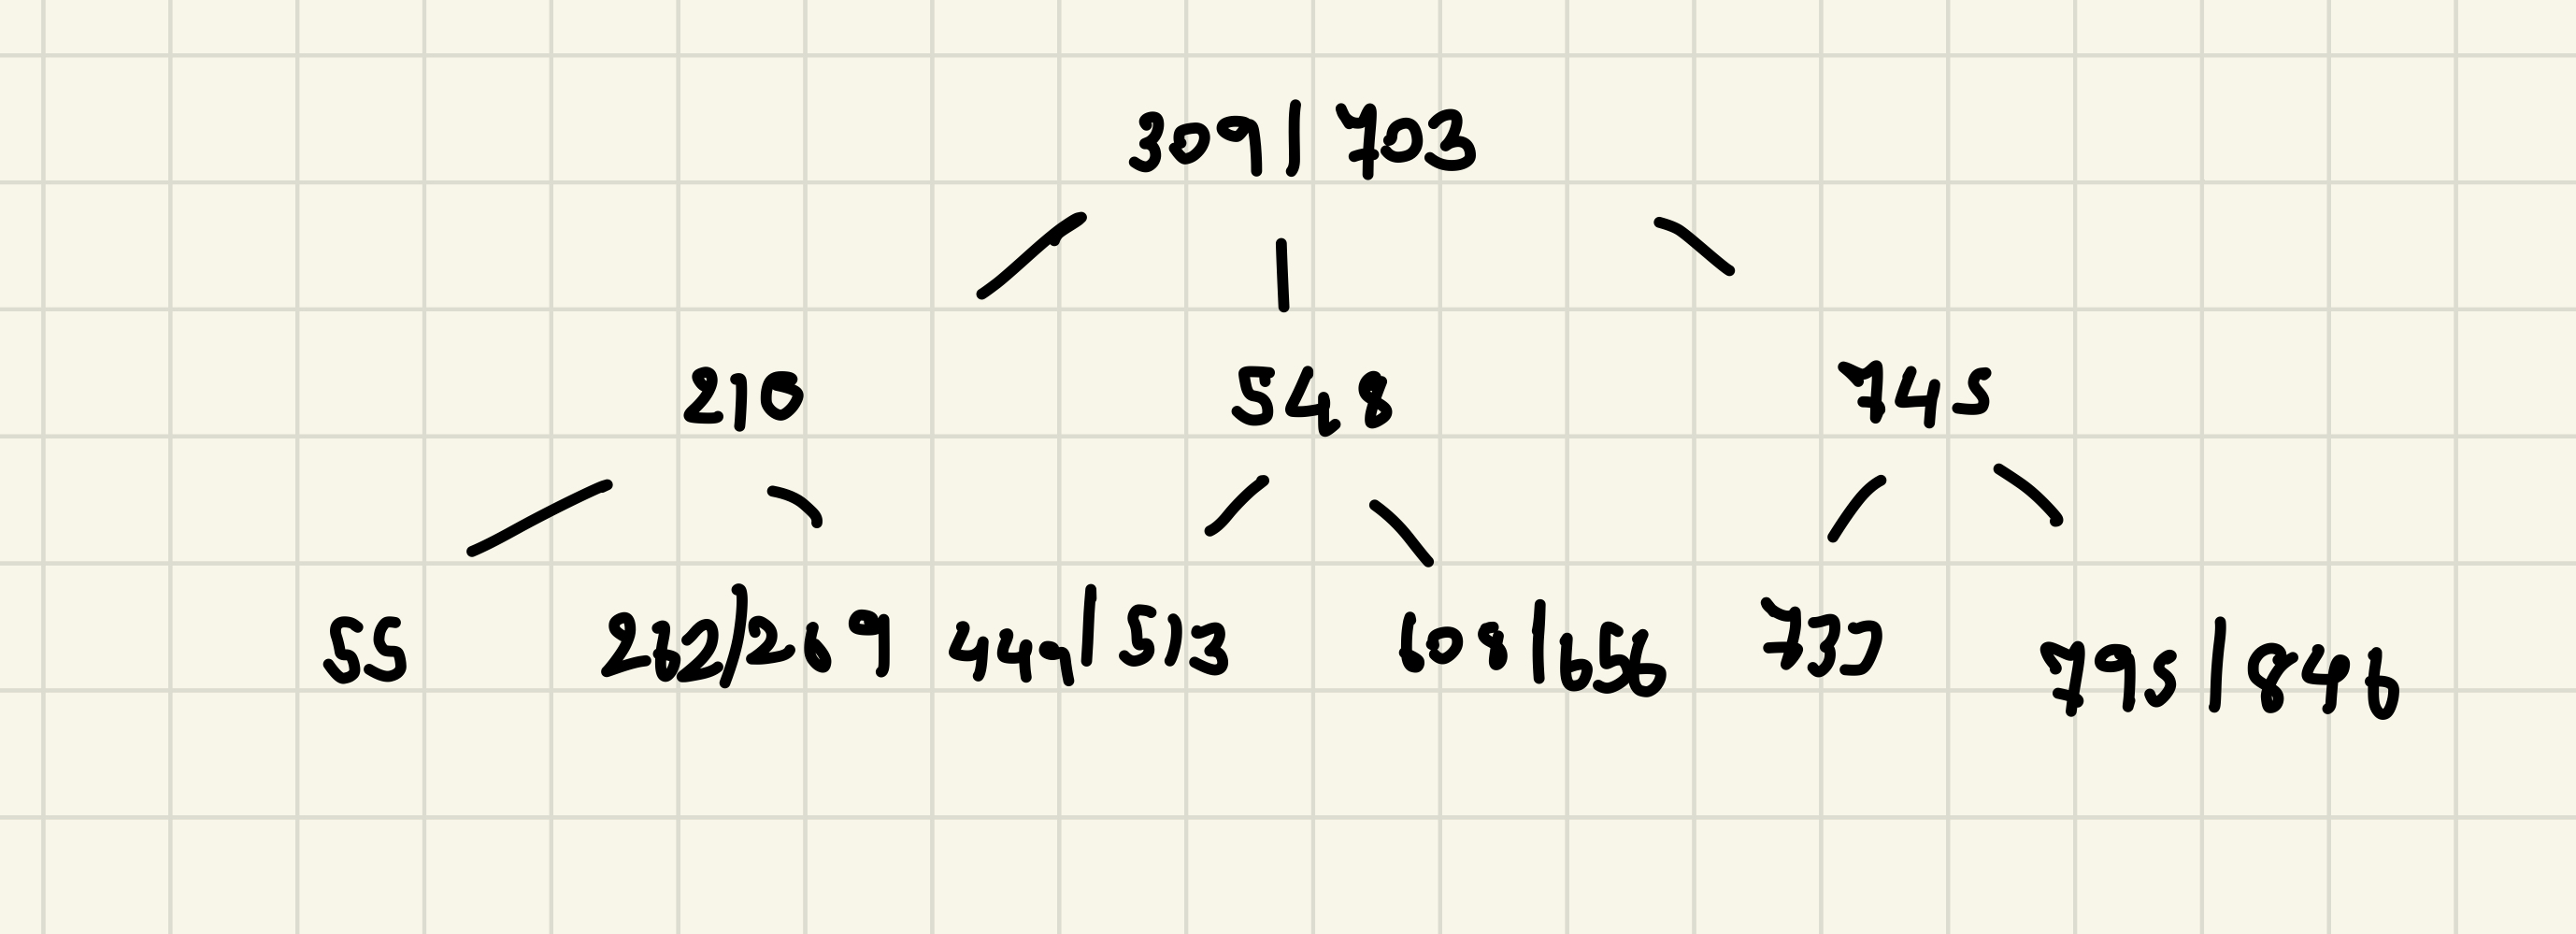
\includegraphics[width=0.9\textwidth,scale=0.5]{tree_insertion.jpeg}
\end{figure}

\section{Key deletion}

\noindent Suppose that we want to delete 309 in \emph{(2,3) tree}, it falls into case 1 which 
we need to steal from sibling.

\begin{figure}[h]
        \centering
        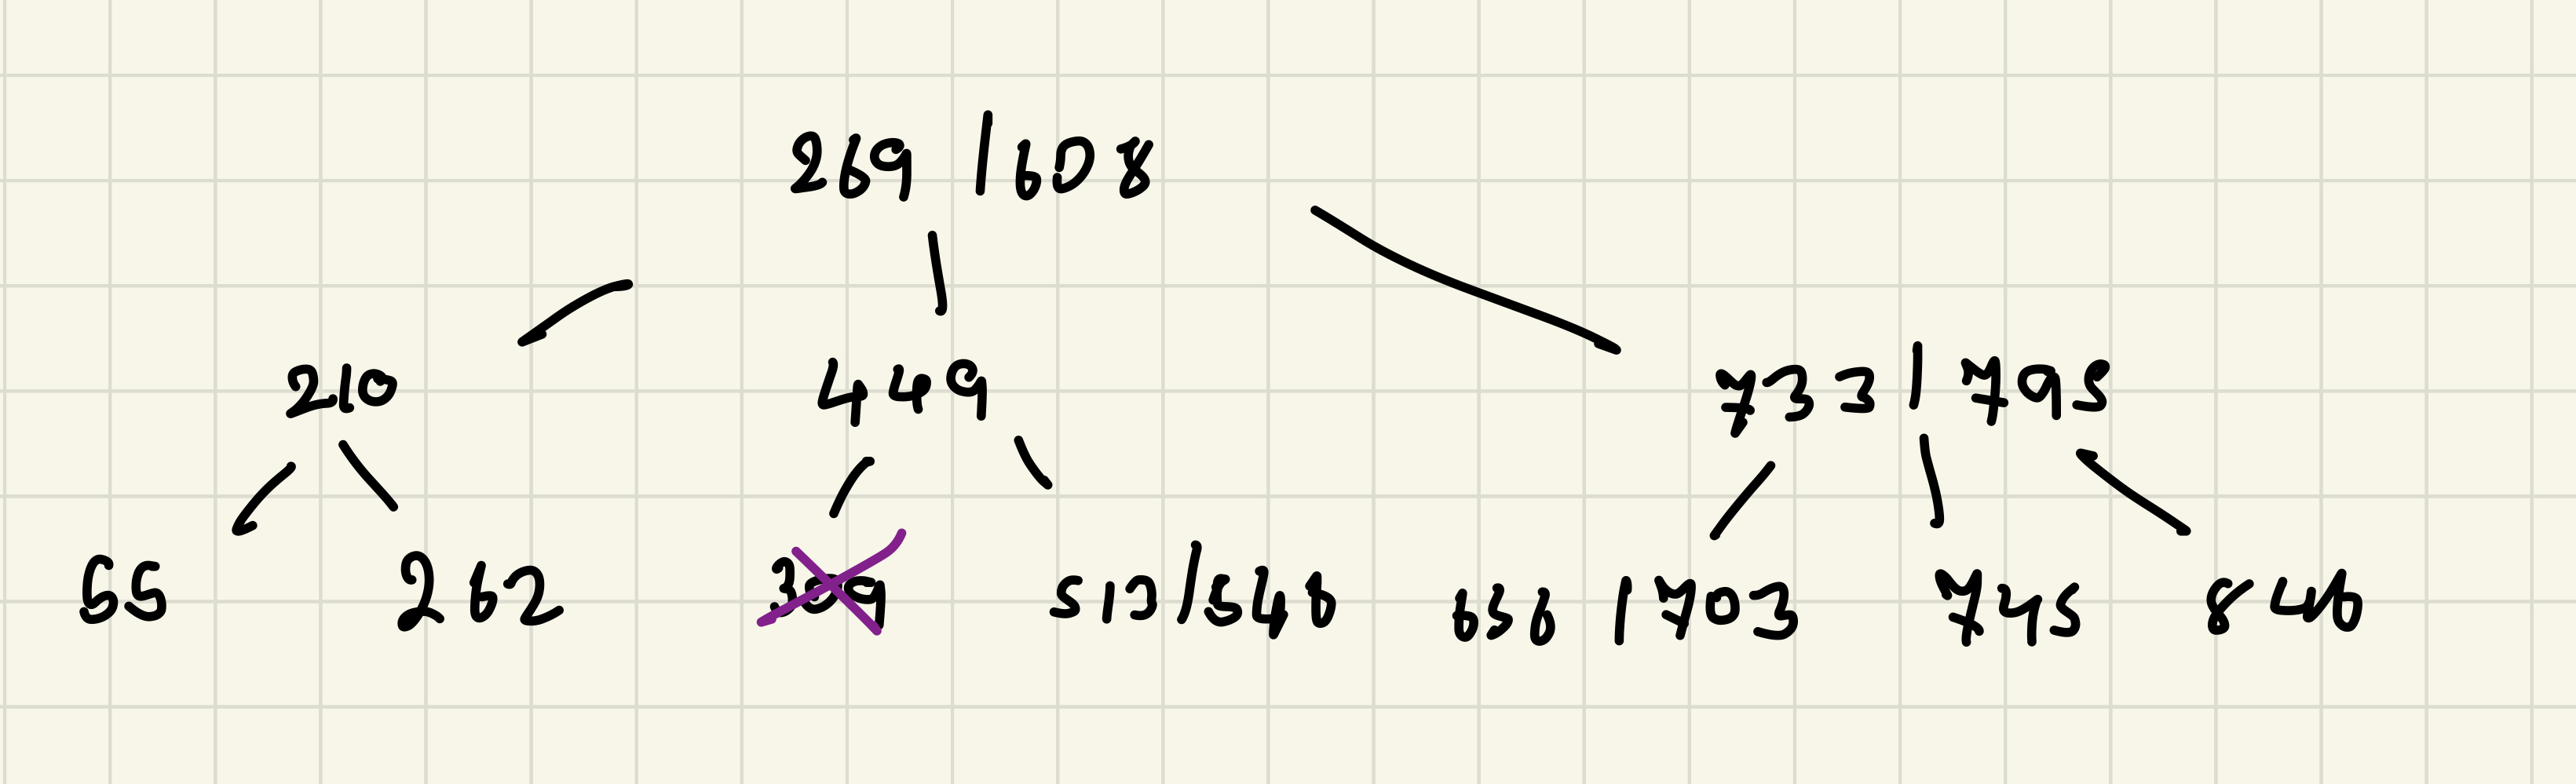
\includegraphics[width=0.8\textwidth,scale=0.5]{tree_deletion_1.jpeg}
        \caption{\label{fig:tree-deletion-1} Unbalanced tree without key 309}
\end{figure}

\begin{figure}[h]
        \centering
        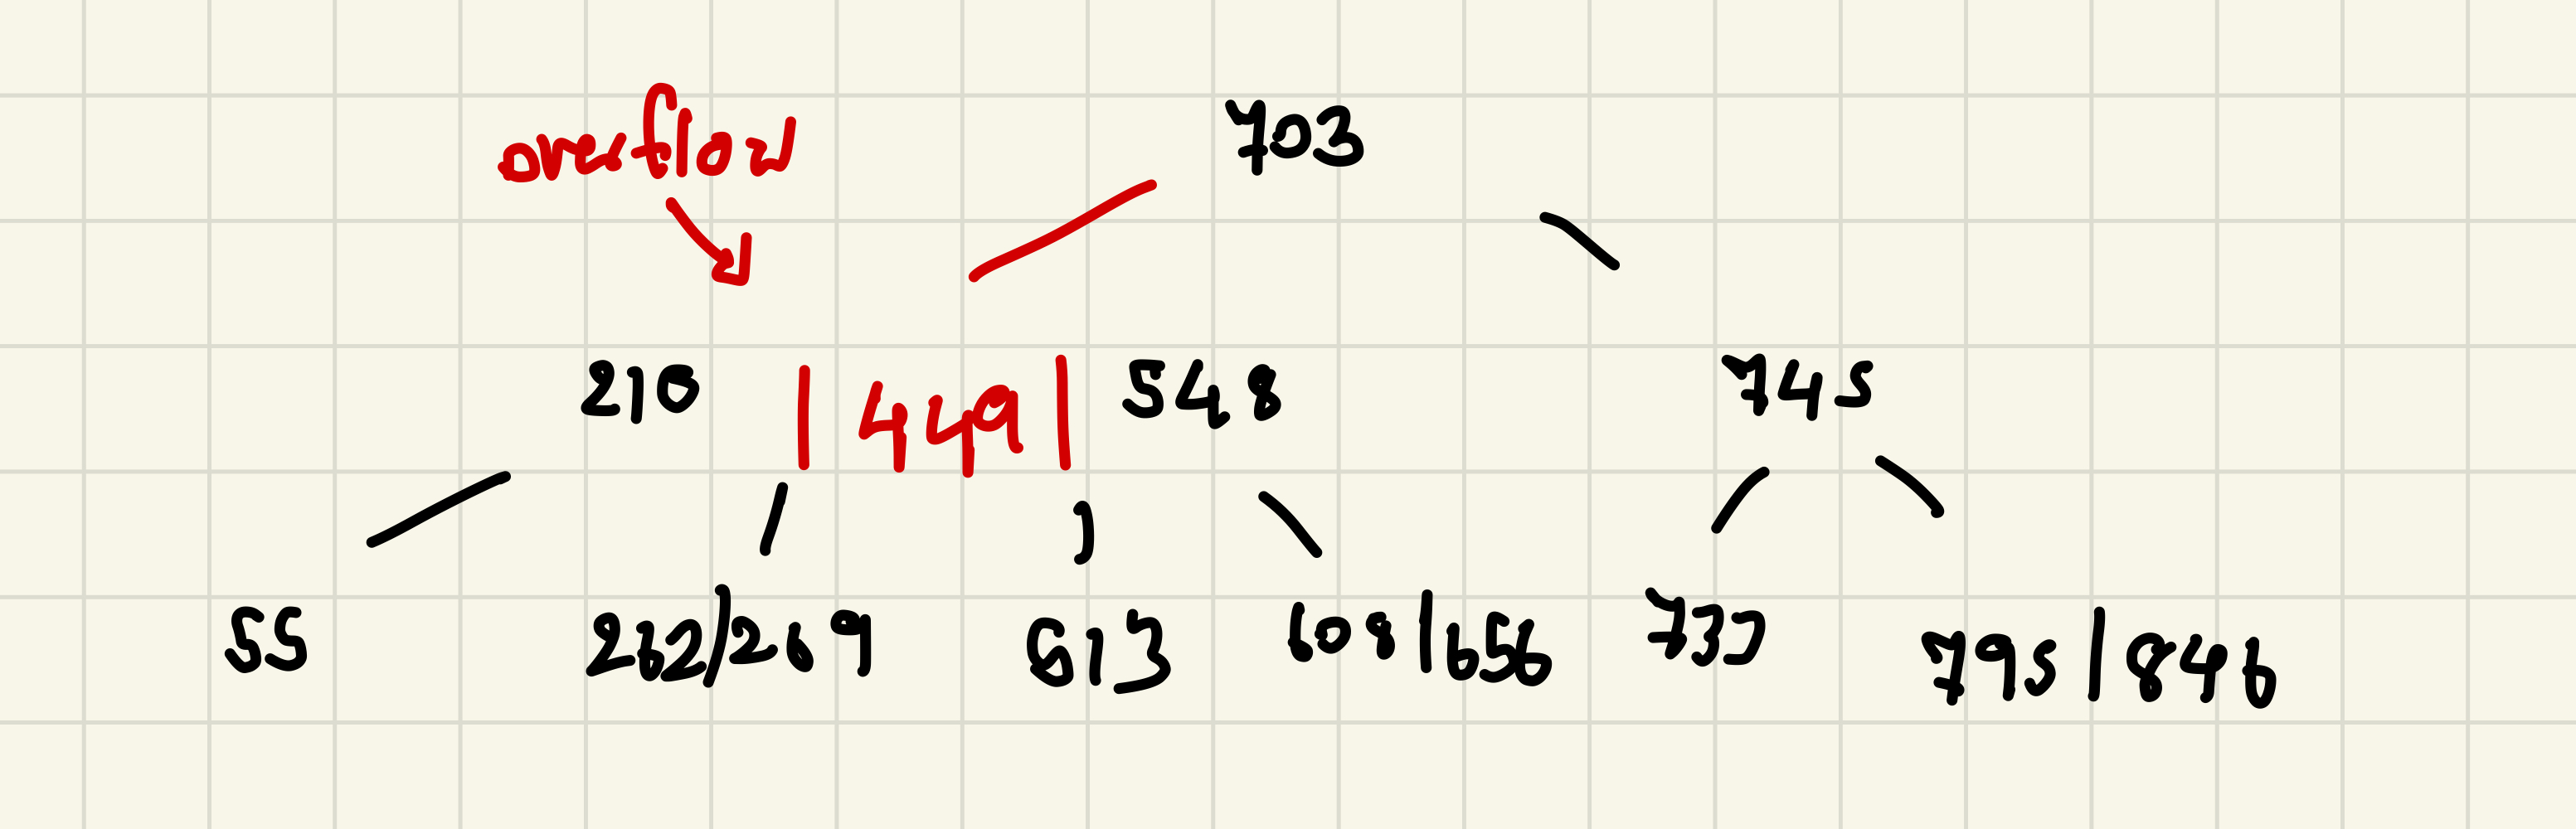
\includegraphics[width=0.8\textwidth,scale=0.5]{tree_deletion_2.jpeg}
        \caption{\label{fig:tree-deletion-2} Balanced tree after finding replacement by stealing}
\end{figure}

As you can see in Figure \ref{fig:tree-deletion-2}, the replacements are 513 and 449 which 513 is the new parent node
that has 449 and 548 as a child nodes. 
\begin{align*}
        \alpha_{\text{me}} = a - 1 + 1
\end{align*} 


\chapter{B-tree speed}
\end{document}
